\documentclass[12pt,a4paper,titlepage,headinclude,bibtotoc]{scrartcl}

%---- Allgemeine Layout Einstellungen ------------------------------------------

% Für Kopf und Fußzeilen, siehe auch KOMA-Skript Doku
\usepackage[komastyle]{scrpage2}
\pagestyle{empty}
\setheadsepline{0.5pt}[\color{black}]
\automark[section]{chapter}


%Einstellungen für Figuren- und Tabellenbeschriftungen
\setkomafont{captionlabel}{\sffamily\bfseries}
\setcapindent{0em}


%---- Weitere Pakete -----------------------------------------------------------
% Die Pakete sind alle in der TeX Live Distribution enthalten. Wichtige Adressen
% www.ctan.org, www.dante.de

% Sprachunterstützung
\usepackage[ngerman]{babel}

% Benutzung von Umlauten direkt im Text
% entweder "latin1" oder "utf8"
\usepackage[utf8]{inputenc}

% Pakete mit Mathesymbolen und zur Beseitigung von Schwächen der Mathe-Umgebung
\usepackage{latexsym,exscale,stmaryrd,amssymb,amsmath}


\usepackage[nointegrals]{wasysym}
\usepackage{eurosym}

% Anderes Literaturverzeichnisformat
%\usepackage[square,sort&compress]{natbib}
\usepackage{hyperref}
% Für Farbe
\usepackage{color}
\usepackage{graphicx}
\usepackage{wrapfig}
\usepackage{subfigure}

% Caption neben Abbildung
\usepackage{sidecap}

% Befehl für "Entspricht"-Zeichen
\newcommand{\corresponds}{\ensuremath{\mathrel{\widehat{=}}}}
% Befehl für Errorfunction
\newcommand{\erf}[1]{\text{ erf}\ensuremath{\left( #1 \right)}}

%Fußnoten zwingend auf diese Seite setzen
\interfootnotelinepenalty=1000

%Für chemische Formeln (von www.dante.de)
%% Anpassung an LaTeX(2e) von Bernd Raichle
\makeatletter
\DeclareRobustCommand{\chemical}[1]{%
  {\(\m@th
   \edef\resetfontdimens{\noexpand\)%
       \fontdimen16\textfont2=\the\fontdimen16\textfont2
       \fontdimen17\textfont2=\the\fontdimen17\textfont2\relax}%
   \fontdimen16\textfont2=2.7pt \fontdimen17\textfont2=2.7pt
   \mathrm{#1}%
   \resetfontdimens}}
\makeatother

%Honecker-Kasten mit $$\shadowbox{$xxxx$}$$
\usepackage{fancybox}

%SI-Package
\usepackage{siunitx}

%keine Einrückung, wenn Latex doppelte Leerzeile
\parindent0pt

%Bibliography \bibliography{literatur} und \cite{gerthsen}
%\usepackage{cite}
\usepackage{babelbib}
\selectbiblanguage{ngerman}

\begin{document}

\begin{titlepage}
\centering
\textsc{\Large Praktikum zur Einführung in die physikalische Chemie,\\[1.5ex] Universität Göttingen}

\vspace*{2cm}

\rule{\textwidth}{1pt}\\[0.5cm]
{\huge \bfseries
  V5: Leitfähigkeit\\[1.5ex]
  wässriger Elektrolyte}\\[0.5cm]
\rule{\textwidth}{1pt}

\vspace*{1cm}


\begin{Large}
\begin{tabular}{ll}
Durchführende: &  Alea Tokita, Julia Stachowiak\\
Assistentin: & Annemarie Kehl\\
 Versuchsdatum: & 01.02.2016\\
 Datum der ersten Abgabe: & 08.02.2016\\

\end{tabular}
\end{Large}

\vspace*{1.5cm}

\begin{Large}
\fbox{
  \begin{minipage}[t][5cm][t]{7cm} 
  Messwerte:\\
  
Literaturwert: \\

  
  
  \end{minipage}
}
\end{Large}

\end{titlepage}

\tableofcontents

\newpage

\section{Theorie}
Ziel des Versuchs ist es, die Grenzleitfähigkeiten eines starken und eines schwachen Elektrolyten zu bestimmen. Dies erfolgt über Leitfähigkeitsmessungen verschieden konzentrierter Lösungen des Elektrolyten.
\subsection{Elektrolyt}
Unter einem wässrigen Elektrolyten $\mathrm{M}_{v+}\mathrm{A_{v-}}$ versteht man einen Stoff, welcher im Wasser in positive und negative Ionen (Kationen und Anionen) dissoziiert. Es wird dabei zwischen schwachen und starken Elektrolyten unterschieden. Ein starker Elektrolyt dissoziiert vollständig in Anionen und Kationen, wobei $v_+$ und $v_-$ die stöchiometrischen Koeffizienten der Dissoziationsreaktion sind und die Ionen verschiedene Ladungszahlen $z_+\mathrm{bzw} z_-$ tragen.\\\\
Ein schwacher Elektrolyt dissoziiert nur teilweise in Lösung, der Dissoziationsgrad $\alpha $ gibt den Bruchteil der eingesetzten Stoffmenge $n_0$ der dissozierten Moleküle an. Dabei liegen $v_{\pm } \cdot \alpha \cdot n_0$ Mol an postiven und negativen Ionen vor, da gilt:
\begin{align}
\alpha = \dfrac{n_0 - n_u}{n_0}
\end{align} 
Wobei $n_u$ die Stoffmenge der undissoziierten Teilchen angibt.
\subsection{Leitfähigkeit}
Ein Maß für die Leitfähigkeit einer Lösung und demzufolge auch des darin enthaltenen Elektrolyten, ist ihr elektrischer Widerstand $R$. Nach dem Ohmschen Gesetzt gilt folgende Abhängikeit von der elektrischen Spannung $U$ under der Stromstärke $I$:
\begin{align}
\dfrac{U}{I} = R = \mathrm{const}.
\end{align}
$R$ ist dabei abhängig von den geometrischen Dimensionen des Stromleiters. Im einfachsten Fall eines metallischen Leiters der Länge $l$ und Querschnittsfläche $A$, ist der Widerstand umso stärker je größer $A$ und je kleiner $l$ ist. Demnach ist der Widerstand durch die Abmessungen sowie andererseits durch eine Materialkonstante, der spezifische Wiederstand $\rho $ gegeben:
\begin{align}
R = \rho \dfrac{l}{A} \quad \quad  [R]=  \mathrm{m}
\end{align} 
%\Ohm !!!
Da ein Material den Strom umso besser leitet, je geringer sein Widerstand ist, verwendet man den Leitwert $L$, um seine charakteristischen Eigenschaften zu beschreiben. Die Erfassung der geometrischen Abmessungen der Messzelle ist aufgrund der komplizierten Ionenwanderung sehr schwierig, daher wird die Proportionalitätsfaktor $Z$ zwischen $R$ und $\rho$ eingeführt. Des weiteren wird der reziproke Wert des spezifischen Widerstands als $\kappa$ bezeichnet:
\begin{align}
L = \dfrac{1}{R} = \dfrac{1}{\rho } \dfrac{A}{l} = \dfrac{\kappa }{Z}
\end{align} 
Da die Leitfähigkeit von der Einwaagekonzentration abhängig ist, definiert man die molare Leitfähigkeit $\Lambda$ einer Elektrolytlösung mit der Einwaagekonzentration $c^*$:
\begin{align}
\Lambda = \dfrac{\kappa}{c^*}
\end{align}

\subsection{Kohlrausches Quadratwurzelgesetz, Grenzleitfähigkeit}
Ionen haben eine unterschiedliche Beweglichkeit und unterschiedliche Ladungen, daher tragen sie in unterschiedlicher Weise zur Gesamtleitfähigkeit bei. Daher ist die molare Leitfähigkeit wiederum Konzentrationsabhängig, dies gilt selbst bei vollständiger Dissoziation, da sich Ionen in ihrer Bewegung gegenseitig Beeinflussen.\\
Eine wichtige Bezugsgröße ist die molare Grenzleitfähigkeit $\Lambda^0$, welche der bei unendlicher Verdünnung gemessenen molaren Leitfähigkeit entspricht. Sie kann aus einer Extrapolation $ \lim \limits_{c \rightarrow 0 } \Lambda = \Lambda ^0$ bestimmt werden und setzt sich additiv aus den Anteilen einzelner Ionensorten zusammen.\\\\
Das nach Kohlrausch benannte Quadratwurzelgesetz beschreibt die Konzentrationsabhängigkeit der molaren Leitfähigkeit:
\begin{align}
\Lambda = \Lambda ^0 - \kappa \cdot \sqrt{c}
\end{align}
\subsection{Unvollständige Dissoziation, Ostwaldsches Verdünnungsgesetzt}
Die Konzentrationsabhängigkeit der molaren Leitfähigkeit ist bei schwachen Elektrolyten wesentlich stärker. Da sie nicht vollständig dissoziieren gilt das Kohlrausche Quadratwuzelgesetz nicht. Die Leitfähigkeit ist stark durch die Gleichgewichtskonzentration bestimmt.\\\\
Stellt man das Massenwirkungsgesetzt für die Dissoziation eines schwachen Elektrolyten auf und setzt für die Konzentration des Elektrolyten deren Verhältnis der Einwaagekonzentration $c^*$ zum Dissoziationsgrad ein, erhält man folgenden Ausdruck:
\begin{align}
K_\mathrm{S} = \dfrac{\alpha ^2}{1-\alpha } \cdot \dfrac{c^*}{c^0}
\end{align}
Zur Leitfähigkeit tragen nur die Ionen des dissoziierten Elektrolyten bei. Bei sehr kleinen Einwagekonzentrationen ($c^* \rightarrow 0$) dissoziieren schwache Elektrolyte vollständig, jedoch ist dann auch die Ionenkonzentration sehr klein. Auch bei höheren Einwaagekonzentrationen ist die Ionenkonzentration aufgrund des niedrigen Dissoziationsgrades die Ionenkonzentration klein. Dementsprechend kann man in guter Näherung annehmen, dass die Leitfähigkeit proportional zur Zahl der dissoziierten Moleküle und damit proportional zum Dissoziationsgrad $\alpha$ ist. Somit gilt näherungweise für die molare Leitfähigkeit:
\begin{align}
\lambda = \alpha \cdot \Lambda ^0 
\end{align}    
Setzt man dies Beziehung in Gleichung ein, erhält man das Ostwaldsche Verdünnungsgesetzt:
\begin{align}
K_\mathrm{S} = \dfrac{c^* \cdot \Lambda ^2}{c^0 \cdot \Lambda ^0 \cdot (\Lambda ^0 - \Lambda)}
\end{align} 
 Aus der Auftragung von $\dfrac{1}{\Lambda}$ gegen $c^* \cdot \Lambda$ lässt sich die Säurekonstante und die Grenzleitfähigkeit ermitteln, entsprechend der Gleichung umgestellt:
\begin{align}
\dfrac{1}{\Lambda} = \dfrac{1}{\Lambda ^0} * \dfrac{c^* \cdot \Lambda }{K_\mathrm{S} \cdot (\Lambda ^0)^2 \cdot c^\circ}
\end{align}

\newpage
\section{Durchführung}
\section{Versuchsaufbau}
\begin{figure} [h!]
\begin{center}
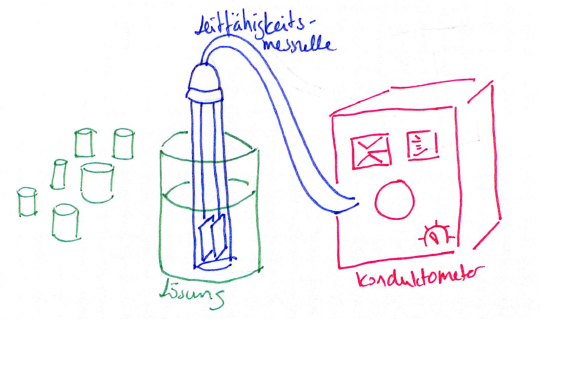
\includegraphics[scale=1]{Versuchsaufbau.png} \end{center}
\caption {Versuchsaufbau}
\end{figure}

Gemessen wird der elektrische Leitwert $L$ der Elektrolytlösung in der elektrochemischen Zelle eines Konduktometers. Dies erfolgt im genaueren mithilfe einer Wheatstone-Brückenschaltung. Die verwendeten Zellen zeigen bei Abgleich der Messbrücke auf den Zeigerauschlag null direkt den Leitert $L$ an. Auch die Zellkonstante $Z$ ist bereits gegeben.
\section{Versuchdurchführung}
Da die Konzentrationsabhängigkeit der molaren Leitfähigkeit von Kaliumchlorid- und Essigsäurelösungen bestimmt werden sollen, werden zunächst Essigsäure- und Kaliumchloridlösungen der Konzentration $0,1 {~}\mathrm{M}$, $0,01{~}\mathrm{M}$ und $0,001{~}\mathrm{M}$ hergestellt. Dies erfolgt über das Verdünnen von $0,1{~}\mathrm{M}$ Lösungen der Elektrolyten.\\\\
Bei den Messungen wird mit der Messung der Eigenleitfähigkeit von destillierten Wasser, welches zum Verdünnen benutzt wurde, begonnen, um eine Abschätzung des Einflusses der Eigenleitfähigkeit des Wassers auf die Messergebnisse zu ermöglichen. Anschließend wird bei den Messungen der Elektrolytlösungen die Lösung der geringsten Konzentration zuerst gemessen. Die Leifähigkeit der Lösungen wird mindestens fünfmal gemessen und zu jeder Messung die Temperatur der Lösung notiert. Beim Messen muss darauf geachtet werden, dass Stellrad am Konduktometer nur langsam und vorsichtig zu bewegen.\\\\
Vor der Messung werden Becherglas, Tauchelektrode und das Thermometer mehrfach mit destilliertem Wassern und anschließend mit der zu messenden Lösung gespült. Zur Messung wird das Becherglas so weit mit der Messlösung gefüllt, dass dass die Tauchglocke der Elektroden vollständig bedeckt ist und zur vollständigen Benetzung vorsichtig mit der Elektrode gerührt. Zwischen den Messungen wird die Elektrode gründlich mit destilliertem Wasser gespült.



\newpage

\section{Auswertung}

Aus den Messungen werden die Mittelwerte des Leitwertes $L$ bestimmt und die Eigenleitfähigkeit des Wassers davon abgezogen. Mit der Zellkonstante $Z$ der Leitfähigkeits-Messzelle wird die spezifische Leitfähigkeit $\kappa$ für jede Lösung errechnet:\\

\begin{equation}
\kappa = \frac{Z}{R} = Z \cdot L
\end{equation}

Daraus ergibt sich die molare Leitfähigkeit $\Lambda$ der Lösungen:\\

\begin{equation}
\Lambda = \frac{\kappa}{c^*}
\end{equation}

Für die Auftragungen wird die molare Leitfähigkeit bei der gemessenen Temperatur auf die Leitfähigkeit bei $25^\circ\text{C}$ umgerechnet, der Koeffizient $m$ ist für die beiden Lösungen unterschiedlich:\\

\begin{equation}
\Lambda (25^\circ\text{C}) = \Lambda(\Omega) \cdot [1+ m \cdot (25- (\Omega/^\circ\text{C}))]
\end{equation}\\

{\centering
$m_{\mathrm{KCl}} = 2,31 \cdot 10^{-2}$ für $0,1\, \mathrm{M} > c_s > 0,001\, \mathrm{M}$\\
$m_{\mathrm{HAc}} = 1,44 \cdot 10^{-2}$ für $0,1\, \mathrm{M} > c_s > 0,001\, \mathrm{M}$\\}



\subsection{Bestimmung von $\Lambda^0$ und $K_{\mathrm{S}}$ für Essigsäure}

Für den schwachen Elektrolyten kann das Ostwaldsche Verdünnungsgesetz umgeformt werden:\\

\begin{equation}
\frac{1}{\Lambda} = \frac{1}{\Lambda^0} + \frac{c^* \cdot \Lambda}{K_{\mathrm{S}} \cdot (\Lambda^0)^2 \cdot c^0}
\end{equation}

Aufgetragen wird $\frac{1}{\Lambda}$ gegen $\frac{c^* \cdot \Lambda}{c^0}$.
Der reziproke Wert für die Grenzleitfähigkeit $\Lambda^0$ ergibt somit durch Extrapolation des Graphen als Schnittpunkt mit der Abszisse.\\
Als Steigung $m$ bleibt  $m = \frac{1}{K_{\mathrm{S}} \cdot (\Lambda^0)^2 }$.\\
Die Säurekonstante $K_{\mathrm{S}}$ errechnet sich damit folgendermaßen:\\

\begin{equation}
K_{\mathrm{S}} = \frac{1}{m \cdot (\Lambda^0)^2}
\end{equation}

Folgende Werte ergeben sich für die Auftragung:\\

\begin{table} [h]
\centering 
\begin{tabular}{|p{4cm}||p{4cm}|p{4cm}|p{4cm}|}
\hline
& $\frac{1}{\Lambda(25^\circ\text{C})}$ in $\frac{\mathrm{mol}}{\mathrm{S} \cdot \mathrm{cm}}$ & $\frac{c^*}{c^0} \cdot \Lambda(25^\circ\text{C})$ in $\frac{\mathrm{S} \cdot \mathrm{cm}}{\mathrm{mol}}$ & $\frac{1}{\Lambda}$ in $\frac{\mathrm{mol}}{\mathrm{S} \cdot \mathrm{cm}}$\\
\hline
0,1 M & & & \\
\hline
0,01 M & & & \\
\hline
0,001 M & & & \\
\hline
\end{tabular}
\end{table}

Daraus ergibt sich:\\

$K_{\mathrm{S}} = 2,5 \cdot 10^{-5}$\\
$\Lambda^0 = 0,3\, \frac{\mathrm{mol}}{\mathrm{S} \cdot \mathrm{cm}}$\\





\subsection{Bestimmung von $\Lambda^0$ für Kaliumchlorid}

Für den starken Elektrolyten Kaliumchlorid wird das Kohlrausche Quadratwurzelgesetz $\Lambda$ gegen $\sqrt{c}$ aufgetragen:\\

\begin{equation}
\Lambda = \Lambda^0 - k \cdot \sqrt{c}
\end{equation}

$\Lambda^0$ ergibt sich ebenfalls aus Extrapolation als Schnittpunkt mit der Abszisse.

Für die Auftragung ergeben sich als Werte:\\


\begin{table} [h]
\centering 
\begin{tabular}{|p{4cm}||p{4cm}|p{4cm}|}
\hline
& $\Lambda(25^\circ\text{C})$ in $\frac{\mathrm{S} \cdot \mathrm{cm}}{\mathrm{mol}}$ & $\sqrt{c}$ in $\mathrm{mol^{\frac{1}{2}}} \cdot \mathrm{l^{- \frac{1}{2}}}$\\
\hline
0,1 M & &  \\
\hline
0,01 M & &  \\
\hline
0,001 M & &  \\
\hline
\end{tabular}
\end{table}

Für $\Lambda^0$ ergibt sich somit:\\
$\Lambda^0 = 15$\\

\section{Fehlerrechnung}

\subsection{absolute Fehler}
Die absoluten Fehler bzw. Messungenauigkeiten der Geräte betragen:\\

\begin{table} [h]
\centering 
\begin{tabular}{p{4cm}p{4cm}}
$\Delta$ Temperatur & $= 0,1^\circ\text{C}$ \\
$\Delta$ Kolben &$= 1$ mL   \\
$\Delta$ Pipette &  $=0,1$ mL \\
\end{tabular}
\end{table}





\subsection{Fehlerrechnung}
Zuerst wird die absolute Standartabweichung der Leitwerte nach folgender Formel bestimmt:\\

\begin{equation}
s_{\mathrm{N}} = \sqrt{\frac{1}{N-1} \sum_{i=1}^{N}(x_i -\bar{x})}
\end{equation} 

Da es sich um sehr wenige Werte handelt (jeweils 5), muss die Standartabweichung noch mit dem Student'schen t-Faktor multipliziert werden, um den Fehler für $\bar{L}$ zu erhalten:\\

\begin{equation}
\Delta \bar{L} = t_N \cdot \bar{s}_N
\end{equation}

Für $95,5 \%$ Konfidenz und 5 Messwerte beträgt dieser 2,8\protect\footnotemark

\footnotetext{Götz, Eckold: \emph{Grundbegriffe der Fehleranalyse bei praktischen Messungen}, Institut für physikalische Chemie, Uni Göttingen, \textbf{2015}.}


Somit ergeben sich folgende Fehler für $\bar{L}$:

\begin{table} [h]
\centering 
\begin{tabular}{|p{4cm}||p{2cm}|p{2cm}|p{2cm}|}
\hline
& 0,1 M & 0,01 M & 0,001 M \\
\hline
Essigsäure & & & \\
$\bar{L}$ &7,46 & 2,346 & 6,99\\
$s_N$ & 0,055 & 0,019 & 0,11 \\
$\Delta L$ & 0,15& 0,054& 0,31\\
\hline
Kaliumchlorid & & &\\
$\bar{L}$ & 1,756 & 1,98 & 2,04\\
$s_N$& 0,017 & 0,017 & 0,025\\
$\Delta L$ & 0,047& 0,047& 0,070\\
\hline
\end{tabular}
\end{table}

\subsection{Fehlerfortpflanzung für $\Lambda$}
$\Lambda$ wird in den Rechnungen weiterverwandt und aufgetragen, sodass eine Fehlerfortpflanzung nach Gauß durchgeführt werden muss. Die Formel dafür lautet:\\

\begin{equation}
\Delta f = \sqrt{\sum_i \left(\frac{\delta f}{\delta x_i}\right)^2_j \cdot \Delta x_i^2}
\end{equation}

Für $\kappa = Z \cdot L$ und $c^* =\frac{n}{V}$ ergibt sich aus $\Lambda = \frac{\kappa}{c^*}= \frac{Z \cdot L \cdot V}{n}$ folgende Fehlerfortpflanzung:\\

\begin{equation}
\Delta \Lambda = \sqrt{\left(\frac{Z \cdot V}{n}\right)^2 \cdot {\Delta L}^2 + \left(\frac{Z \cdot L}{n}\right)^2 \cdot \Delta V^2}
\end{equation}

Daraus ergeben sich folgende Fehler für $\Delta L$, welche als Fehlerbalken in die Auftragungen eingetragen werden:\\

\begin{table} [h]
\centering 
\begin{tabular}{|p{4cm}||p{4cm}|p{4cm}|p{4cm}|}
\hline
& 0,1 M & 0,01 M & 0,001 M \\
\hline
$\Delta L$ Essigsäure  & $100,6527 \approx 1\cdot 10$ & $362,21 \approx 4 \cdot 10^2 $& $20776,39 \approx 2 \cdot 10^4$ \\
\hline
$\Delta L$ Kaliumchlorid &$31,5 \approx 3 \cdot 10$ & $315,2 \approx 3 \cdot 10^2$ & $4692,4 \approx 5 \cdot 10^3$\\
\hline
\end{tabular}
\end{table}

\subsection{Fehler für $\Lambda^0$ und $K_{\mathrm{S}}$ aus der Auftragung}

Durch die eingezeichneten Grenzgeraden kann aus der maximalen und minimalen Steigung der absolute Fehler für $\Lambda^0$ bestimmt werden:\\


Bestimmung des Fehlers für $K_{\mathrm{S}}$:\\


\subsection{Diskussion systematischer Fehler}

unendliche Verdünnung ungleich c gleich 0, sondern kurz davor (falscher wert)(etwas zu klein)
Auftragung von 3 Werten sehr wenig und ungenau -> Auftragung sehr fehlerhaft

Ablesefehler Messgeräte
Eigendissoziation des Wassers
Einfluss Temperatur berücksichtigt/nicht berücksichtigt?



\section{Vergleich mit Literaturwerten}

\subsection{Diskussion}

\newpage

\section{Literaturverzeichnis}
\begin{flushleft}
1 \quad Gerd Wedler: \emph{Lehrbuch der physikalischen Chemie}, 5. Aufl., WILEY-VCH Verlag GmbH Co. KGaA, Weinheim, \textbf{2004}.\\
\vspace{0,5 cm}
2\quad Götz, Eckold: \emph{Sriptum zur Einführung in die physikalische Chemie}, Institut für physikalische Chemie, Uni Göttingen, \textbf{2015}.\\
\vspace{0,5 cm}
3 \quad \emph{Skriptum für das Praktikum zur Einführung in die Physikalische Chemie}, Institut für physikalische Chemie, Uni Göttingen, \textbf{2015}.\\
\end{flushleft}



\end{document}



